\documentclass{article}
\usepackage{tikz}
\usetikzlibrary{positioning, shapes.geometric, arrows.meta}

\begin{document}

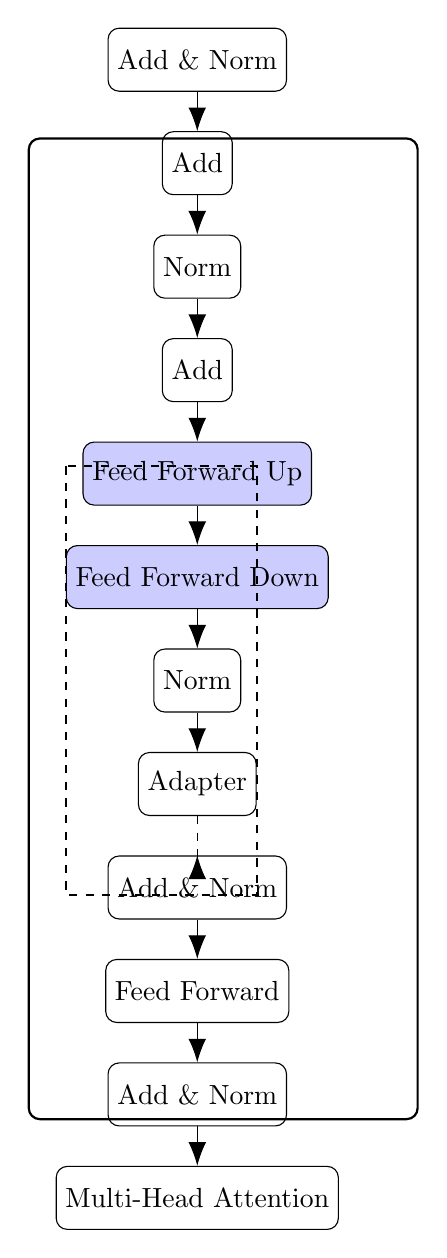
\begin{tikzpicture}[node distance=5mm,
    block/.style={draw, rounded corners, minimum height=8mm},
    arrow/.style={-{Latex[length=3mm]}},
    dashed arrow/.style={-{Latex[length=3mm]}, dashed}
]

% Define nodes
\node[block] (add_norm) {Add \& Norm};
\node[block, below=of add_norm] (add) {Add};
\node[block, below=of add] (norm) {Norm};
\node[block, below=of norm] (add2) {Add};
\node[block, below=of add2, fill=blue!20] (ff_up) {Feed Forward Up};
\node[block, below=of ff_up, fill=blue!20] (ff_down) {Feed Forward Down};
\node[block, below=of ff_down] (norm2) {Norm};
\node[block, below=of norm2] (adapter) {Adapter};
\node[block, below=of adapter] (add_norm2) {Add \& Norm};
\node[block, below=of add_norm2] (ff) {Feed Forward};
\node[block, below=of ff] (add_norm3) {Add \& Norm};
\node[block, below=of add_norm3] (attn) {Multi-Head Attention};

% Draw arrows
\draw[arrow] (add_norm) -- (add);
\draw[arrow] (add) -- (norm);
\draw[arrow] (norm) -- (add2);
\draw[arrow] (add2) -- (ff_up);
\draw[arrow] (ff_up) -- (ff_down);
\draw[arrow] (ff_down) -- (norm2);
\draw[arrow] (norm2) -- (adapter);
\draw[dashed arrow] (adapter) -- ++(0,-10mm) -| (add_norm2);
\draw[arrow] (add_norm2) -- (ff);
\draw[arrow] (ff) -- (add_norm3);
\draw[arrow] (add_norm3) -- (attn);

% Draw dashed box around the adapter section
\draw[dashed, thick] ([shift={(0,1)}]ff_down.north west) rectangle ([shift={(0,-1)}]adapter.south east);

% Draw the outer rectangle
\draw[thick, rounded corners] ([shift={(-1,-1)}]add_norm.west) rectangle ([shift={(1,1)}]attn.east);

\end{tikzpicture}

For the individual adapter predictions, we use a Transformer-based model with adapter layers inserted after the feed-forward layer of the Transformer as proposed by \citet{pfeiffer-etal-2021-adapterfusion}.

\end{document}